
\chapter{Git}

%% link to git cheatsheet
\href{https://training.github.com/downloads/github-git-cheat-sheet.pdf}{GitHub Cheatsheet}

\section{About Git}

\subsection{About version control and Git}

\begin{definitionblock}[Version control]
    A version control system, or VCS, tracks the history of changes as people and teams collaborate on projects together. As developers make changes to the project, any earlier version of the project can be recovered at any time.
\end{definitionblock}

Developers can revew project history to find out:
\begin{itemize}
    \item Which changes were made?
    \item Who made the changes?
    \item When were the changes made?
    \item Why were changes needed?
\end{itemize}

In a \textbf{distributed version control system (DVCSs)}, every developer has a full copy of the prokect and project history. They don't need a constant connection to a central repository. \texttt{Git} is the most popular distributed version control syste. It is commonly used for both open source and commercial software development, with significant benefits for individuals, teams and businesses. 

\begin{tipsblock}
    \begin{itemize}
        \item \textbf{Git lens} is used to see the entire timeline of the project, including decisions, changes and progressions. From the moment they access the history of a project, the developer has all the context they need to understand it and start contributing.
        \item Developers work in every time zone. With a DVCS like Git, collaboration can happen any time while maintaining source code integrity. Using \textbf{branches}, developers can safely propose changes to production code.
    \end{itemize}
\end{tipsblock}

\subsection{Repositories}

A repository, or Git project, encompasses the entire collection of files and folders associated with a project, along with each file's revision history. The file history appears as \textbf{snapshots} in time called commits. The commits can be organized into multiple lines of development called branches. Because Git is a DVCS, repositories are self-contained units and anyone who has a copy of the repository can access the entire codebase and its history. Using the command line or other ease-of-use interfaces, a Git repository also allows for: interaction with the history, cloning the repository, creating branches, committing, merging, comparing changes across versions of code, and more.

A repository, or Git project, encompasses the entire collection of files and folders associated with a project, along with each file's revision history. The file history appears as snapshots in time called commits. The commits can be organized into multiple lines of development called branches. Because Git is a DVCS, repositories are self-contained units and anyone who has a copy of the repository can access the entire codebase and its history. Using the command line or other ease-of-use interfaces, a Git repository also allows for: interaction with the history, cloning the repository, creating branches, committing, merging, comparing changes across versions of code, and more.

\subsection{GitHub}

GitHub hosts Git repositories and provides developers with tools to ship better code through command line features, issues (threaded discussions), pull requests, code review, or the use of a collection of free and for-purchase apps in the GitHub Marketplace. With collaboration layers like the GitHub flow, a community of 100 million developers, and an ecosystem with hundreds of integrations, GitHub changes the way software is built.

GitHub builds collaboration directly into the development process. Work is organized into repositories where developers can outline requirements or direction and set expectations for team members. Then, using the GitHub flow, developers simply create a branch to work on updates, commit changes to save them, open a pull request to propose and discuss changes, and merge pull requests once everyone is on the same page. 

\subsection{Command Line Interface}

To use Git, developers use specific commands to copy, create, change, and combine code. These commands can be executed directly from the command line or by using an application like GitHub Desktop. Here are some common commands for using Git:

\begin{itemize}
    \item \texttt{git init}: Initializes a new Git repository. Until you run this command inside a repository or directory, it's just a regular folder. Only after you input this does it accept further Git commands.
    \item \texttt{git config}: Short for "configure," this is most useful when you're setting up Git for the first time.
    \item \texttt{git help}: Forgot a command? Type this into the command line to bring up the 21 most common git commands.
    \item \texttt{git status}: We all get a little nervous the first time we commit our changes. This command shows you the status of changes as untracked, modified, or staged.
    \item \texttt{git add}: This does not add new files to your repository. Instead, it brings new files to Git's attention. After you add files, they're included in Git's "snapshots" of the repository.
    \item \texttt{git commit}: Git's most important command. After you make any sort of change, you input this in order to take a "snapshot" of the repository. Usually it goes \texttt{git commit -m "Message here"}.
    \item \texttt{git branch}: Working on multiple features at once? Use this command to list, create, or delete branches.
    \item \texttt{git checkout}: Literally allows you to "check out" a repository that you are not currently inside. This is a navigational command that lets you move to the repository you want to check.
    \item \texttt{git merge}: When you're done working on a branch, you can merge your changes back to the master branch, which is visible to all collaborators.
    \item \texttt{git push}: If you're working on your local computer, and want your commits to be visible online on GitHub as well, you "push" the changes up to GitHub with this command.
    \item \texttt{git pull}: If you're working on your local computer and want your commits to be visible online on GitHub as well, you "push" the changes up to GitHub with this command.
    \item \texttt{git clone}: If you're starting fresh and want to clone an existing repository from GitHub to your local computer, you can use this command to copy the repository to your computer.
    \item \texttt{git remote}: When you clone a repository from GitHub, it automatically creates a connection or "remote" that you can also push changes to.
\end{itemize}

\textbf{\\ Example: Contribute to an existing repository}
\begin{codeblock}[language=bash]
# download a repository on GitHub to our machine
# Replace `owner/repo` with the owner and name of the repository to clone
git clone https://github.com/owner/repo.git

# change into the `repo` directory
cd repo

# create a new branch to store any new changes
git branch my-branch

# switch to that branch (line of development)
git checkout my-branch

# make changes, for example, edit `file1.md` and `file2.md` using the text editor

# stage the changed files
git add file1.md file2.md

# take a snapshot of the staging area (anything that's been added)
git commit -m "my snapshot"

# push changes to github
git push --set-upstream origin my-branch
\end{codeblock}

\textbf{\\ Example: Start a new repository adn publish on GitHub}
\begin{codeblock}[language=bash]
# create a new directory, and initialize it with git-specific functions
git init my-repo

# change into the `my-repo` directory
cd my-repo

# create the first file in the project
touch README.md

# git isn't aware of the file, stage it
git add README.md

# take a snapshot of the staging area
git commit -m "add README to initial commit"

# provide the path for the repository you created on github
git remote add origin https://github.com/YOUR-USERNAME/YOUR-REPOSITORY-NAME.git

# push changes to github
git push --set-upstream origin main
\end{codeblock}

\textbf{\\ Example: Contribute to an existing branch on GitHub}
\begin{codeblock}[language=bash]
# change into the `repo` directory
cd repo

# update all remote tracking branches, and the currently checked out branch
git pull

# change into the existing branch called `feature-a`
git checkout feature-a

# make changes, for example, edit `file1.md` using the text editor

# stage the changed file
git add file1.md

# take a snapshot of the staging area
git commit -m "edit file1"

# push changes to github
git push
\end{codeblock}

\subsection{Models for collaborative development}

THere are two primary ways people collaborate on GitHub:
\begin{itemize}
    \item \textbf{Fork and pull model}: A project owner creates a master repository, and contributors fork that repository to their accounts. They clone the repository to their local machine, make changes, commit them
    \item \textbf{Shared repository model}: In this model, all collaborators have push access to the same repository. This is more common for small teams and organizations.
\end{itemize}

With a shared repository, individuals and teams are explicitly designated as contributors with read, write, or administrator access. This simple permission structure, combined with features like protected branches, helps teams progress quickly when they adopt GitHub.

For an open source project, or for projects to which anyone can contribute, managing individual permissions can be challenging, but a fork and pull model allows anyone who can view the project to contribute. A fork is a copy of a project under a developer's personal account. Every developer has full control of their fork and is free to implement a fix or a new feature. Work completed in forks is either kept separate, or is surfaced back to the original project via a pull request. There, maintainers can review the suggested changes before they're merged. 

\newpage
\section{Pushing commits to a remote repository}

\subsection{About \texttt{git push}}

The \texttt{git push} command takes two arguments.
\begin{itemize}
    \item A remote name, for example, \texttt{origin}
    \item A branch name, for example, \texttt{main}
\end{itemize}

For example, the command \texttt{git push origin main} pushes the commits in the local \texttt{main} branch to the remote repository named \texttt{origin}.
\begin{exampleblock}[Pushing changes to a remote repository]
    \begin{codeblock}[language=bash]
# push changes to the remote repository
git push origin main
    \end{codeblock}
\end{exampleblock}

\subsection{Renaming branches}

To rename a branch, you'd use the same \texttt{git push} command, but you would add one more argument: the name of the new branch. For example:
\begin{exampleblock}[Renaming a branch]
    \begin{codeblock}[language=bash]
# rename the local branch to new-name
git push origin main:new-name
    \end{codeblock}
\end{exampleblock}

This pushes the \texttt{main} branch to the remote repository, but the branch is renamed to \texttt{new-name}.
\begin{tipsblock}
    \begin{itemize}
        \item If you want to delete a branch, you can use the \texttt{--delete} flag with the \texttt{git push} command. For example, \texttt{git push origin --delete new-name} will delete the \texttt{new-name} branch from the remote repository.
        \item If you want to rename the branch you're currently on, you can use the \texttt{-u} flag to set the upstream branch. For example, \texttt{git push -u origin main:new-name} will push the \texttt{main} branch to the remote repository, renaming it to \texttt{new-name}, and set the upstream branch to \texttt{new-name}.
    \end{itemize}
\end{tipsblock}

\newpage
\subsection{Dealing with "non-fast-forward" errors}

If your local copy of a repository is out of sync with, or "behind", the upstream repository you're pushing to, you'll get a message saying \texttt{non-fast-forware updates were rejected}. This means that you must retrieve, or "fetch," the upstream changes, before you are able to push your local changes.

\begin{tipsblock}[Fetching]
    Fetching means retrieving recent commits from a remote repository without merging them into your local branch. This lets you view and compare new changes before deciding how to incorporate them into your work.
\end{tipsblock}

To fetch the changes from the remote repository, you can use the \texttt{git fetch} command. This command retrieves the changes from the remote repository, but it doesn't merge them into your local branch. After fetching the changes, you can merge them into your local branch using the \texttt{git merge} command.

\subsection{Pushing tags}

By default, and without additional parameters, \texttt{git push} sends all matching branches that have the same names as remote branches. 

To push a single tag, you cna issue the same command as pushing a branch:
\begin{codeblock}[language=bash]
git push origin tag-name
\end{codeblock}

To push all your tags, you can type the command:
\begin{codeblock}[language=bash]
git push origin --tags
\end{codeblock}

\subsection{Deleting a remote branch or tag}

The syntax to delete a branch is a bit more arcane at first glance:
\begin{codeblock}[language=bash]
git push origin --delete branch-name
\end{codeblock}

Note that there is a space before the colon. The command resembles the same steps you'd take to rename a branch. However, here, you're telling Git to push \textbf{nothing} into \texttt{branch-name}, effectively deleting it. Because of this, \texttt{git push} deletes the branch on the remote repository. 

\subsection{Remotes and forks}

You can \textbf{fork a repository} on GitHub. 

When you clone a repository you own, you provide it with a remote URL that tells Git where to fetch and push updates. If you want to collaborate with the original repository, you'd add a new remote URL, typically called \texttt{upstream}, to your local Git clone:
\begin{codeblock}[language=bash]
git remote add upstream REMOTE_URL 
\end{codeblock}

Now you can fetch updates and branches from their fork:
\begin{codeblock}[language=bash]
git fetch upstream
# Grab the upstream remote's branches
> remote: Counting objects: 75, done.
> remote: Compressing objects: 100% (53/53), done.
> remote: Total 62 (delta 27), reused 44 (delta 9)
> Unpacking objects: 100% (62/62), done.
> From https://github.com/OCTOCAT/REPO
>  * [new branch]      main     -> upstream/main
\end{codeblock}

When you're done making local changes, you can push your local branch to GitHub and initiate a pull request. 

\section{Getting changes from a remote repository}

\subsection{Options for getting changes}
These commands are very useful when interacting with a remote repository. \texttt{clone} and \texttt{fetch} download remote code from a repository's remote URL to your local computer, \texttt{merge} is used to merge different people's work together with yours, and \texttt{pull} is a combination of \texttt{fetch} and \texttt{merge}.

\subsection{Cloning a repository}
To grab a complete copy of another user's repository, use \texttt{git clone} like this:
\begin{codeblock}[language=bash]    
git clone https://github.com/USERNAME/REPOSITORY.git 
# Clones a repository to your computer
\end{codeblock}

You can choose from different URLs when cloning a repository. While logged in to GitHub, there URLs are available on the main page of the repository when you click \texttt{<> Code}.

\begin{figure}[H]
    \centering
    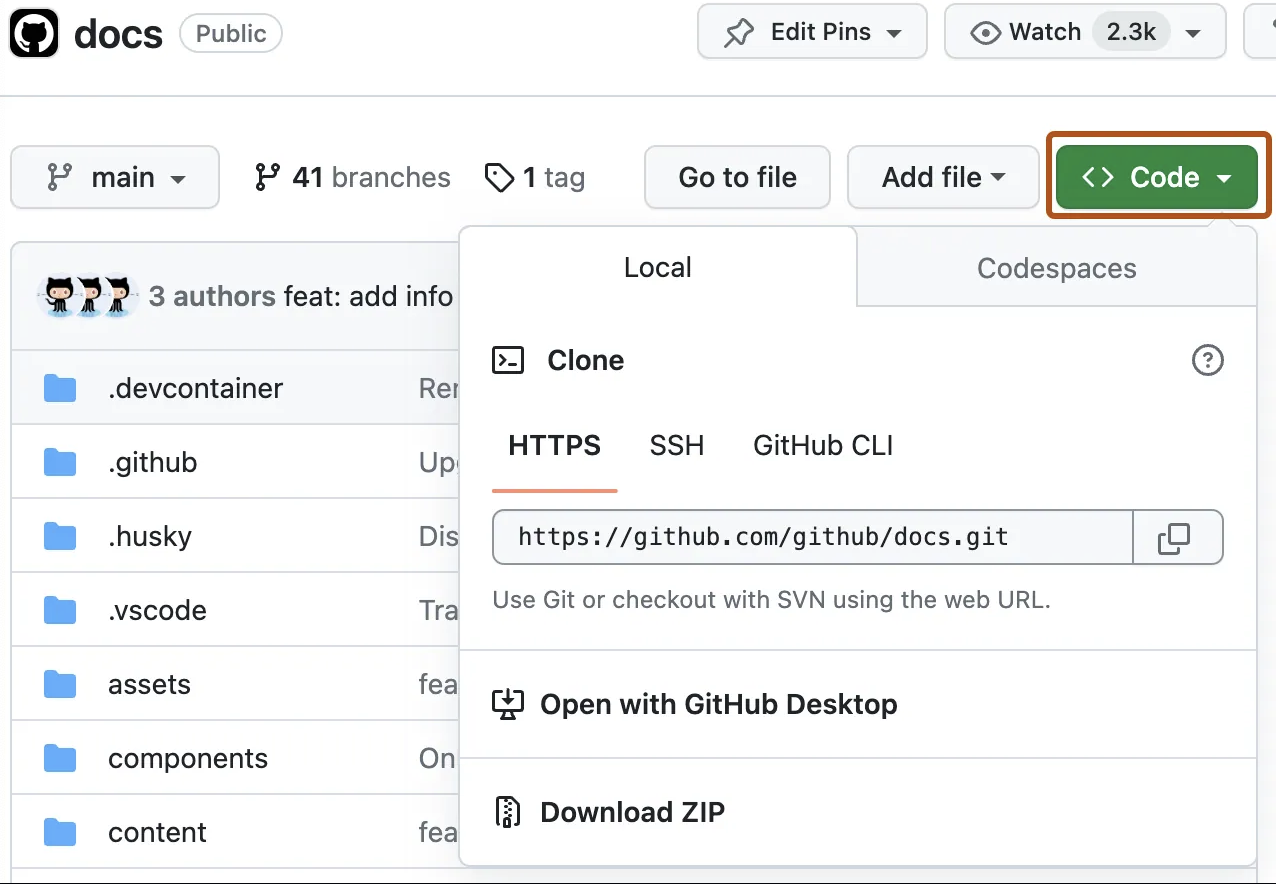
\includegraphics[width=0.8\textwidth]{assets/fig1.png}
\end{figure}

When you run \texttt{git clone}, the following actions occur: 
\begin{itemize}
    \item A new folder called \texttt{repo} is made
    \item It is initialized as a Git repository
    \item A remote named \texttt{origin} is created, pointing to the URL you cloned from  
    \item All of the repository's files and commits are downloaded there 
    \item The default branch is checked out 
\end{itemize}

For every branch \texttt{foo}, a corresponding remote-tracking branch \texttt{refs/remotes/origin/foo} is created in your local repository. You can usually abbreviate such remote-tracking branch names to \texttt{origin/foo}.

\subsection{Fetching changes from a remote repository}

Use \texttt{fit fetch} to retrieve new work done by other people. Fetching from a repository grabs all the new remote-tracking branches and tags without merging those changes into your own branches.

If you already have a local repository with a remote URL set up for the desired project, you can grab all the new information by using \texttt{fit fetch *remotename*} in the terminal.

\begin{codeblock}[language=bash]
git fetch REMOTE-NAME 
# Fetches updates made to a remote repository 
\end{codeblock}

\subsection{Merging changes into your local branch}

Merging combines your local changes with changes made by others.

Typically, you'd merge a remote-tracking branch (i.e., a branch fetched from a remote repository) with your local branch:
\begin{codeblock}[language=bash]
git merge REMOTE-NAME/BRANCH-NAME 
# Merges updates made online with your local work 
\end{codeblock}

\subsection{Pulling changes from a remote repository}

\texttt{git pull} is a convenient shortcut for completing both \texttt{git fetch} and \texttt{git merge} in the same command:
\begin{codeblock}[language=bash]
git pull REMOTE-NAME BRANCH-NAME 
# Grabs online updates and merges them with your local work 
\end{codeblock}

Because \texttt{pull} performs a merge on the retrieved changes, you should ensure that your local work is committed before running the \texttt{pull} command. If you run into a \textbf{merge conflict} you cannot resolve, or if you decide to quit the merge, you can use \texttt{git merge --abort} to take the branch back to where it was in before you pulled. 


\newpage
\section{Dealing with non-fast-forward errors}

Sometimes, Git can't make your change to a remote repository without losing commits. When this happens, your push is refused. 

If another person has pushed to the same branch as you, Git won't be able to push your changes:
\begin{exampleblock}
    \begin{codeblock}[language=bash]
git push origin main
> To https://github.com/USERNAME/REPOSITORY.git
>  ! [rejected]        main -> main (non-fast-forward)
> error: failed to push some refs to 'https://github.com/USERNAME/REPOSITORY.git'
> To prevent you from losing history, non-fast-forward updates were rejected
> Merge the remote changes (e.g. 'git pull') before pushing again. See the
> 'Note about fast-forwards' section of 'git push --help' for details.
    \end{codeblock}
\end{exampleblock}

You can fix this by fetching and merging the changes made on the remote branch with the changes that you have made locally:
\begin{codeblock}[language=bash]
git fetch origin 
# Fetches updates made to an online repository

git merge origin YOUR_BRANCH_NAME
# Merges updates made online with your local work
\end{codeblock}

Or simply use \texttt{git pull} to perform both commands at once:
\begin{codeblock}[language=bash]
git pull origin YOUR_BRANCH_NAME 
# Grabs online updates and merges them with your local work 
\end{codeblock}


\section{Splitting a subfolder out into a new repository}

 You can turn a folder within a Git repository into a brand new repository. 
 \begin{warningblock}
 You need Git version 2.22.0 or later to follow these instructions, otherwise \plaintt{git filter-repo} will not work.
 \end{warningblock}

 If you create a new clone of the repository, you won't lose any of your Git history or changes when you split a folder into a separate repository. However, note that the new repository won't have the branches and tags of the original repository. 

 Steps:
 \begin{enumerate}
    \item Open Terminal.
    \item Change the current working directory to the location where you want to create your new repository.
    \item Clone the repository that contains the subfolder.
    \begin{codeblock}[language=bash]
git clone https://github.com/USERNAME/REPOSITORY-NAME 
    \end{codeblock}
    \item Change the current working directory to your cloned repository.
    \begin{codeblock}[language=bash]
cd REPOSITORY-NAME 
    \end{codeblock}
    \item To filter out the subfolder from the rest of the files in the repository, install \texttt{git-filter-repo}, then run \texttt{git filter-repo} with the following arguments.
    \begin{itemize}
        \item \texttt{FOLDER-NAME}: The folder within your project where you'd like to create a separate repository.
    \end{itemize}
    \begin{codeblock}[language=bash]
git filter-repo --path FOLDER-NAME/
# Filter the specified branch in your directory and remove empty commits 
    \end{codeblock}
    The repository should now only contain the files that were in your subfolder(s).
    
    If you want one specific subfolder to be the new root folder of the new repository, you can use the following command:

    \begin{codeblock}[language=bash]
git filter-repo --subdirectory-filter FOLDER-NAME/
# Filter the specified branch in your directory and remove empty commits
    \end{codeblock}
    \item Create a repository on GitHub.
    \item At the top of your new repository on GitHub's Quick Setup page, click \raisebox{0.3em}{\small$\square$} \hspace{-0.5em} $\square$ to copy the remote repository URL. 
    \begin{figure}[H]
        \centering
        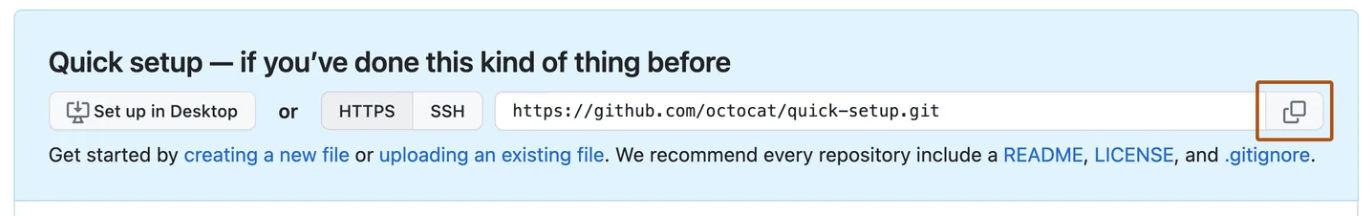
\includegraphics[width=\textwidth]{assets/fig2.png}
    \end{figure}
    \begin{tipsblock}
        For information on the difference between HTTPS and SSH URLs, see \href{https://docs.github.com/en/get-started/git-basics/about-remote-repositories}{About remote repositories}.
    \end{tipsblock}
    \item Add a new remote name with the URL you copied for your repository. For example, \texttt{origin} or \texttt{upstream} are two common choices. 
    \begin{codeblock}[language=bash]
git remote add NEW-REMOTE-NAME URL
    \end{codeblock}
    \item Verify that the remote URL was added with your new repository name.
    \begin{codeblock}[language=bash]
git remote -v
# Verify new remote URL 
> origin  https://github.com/USERNAME/NEW-REPOSITORY-NAME.git (fetch)
> origin  https://github.com/USERNAME/NEW-REPOSITORY-NAME.git (push)
    \end{codeblock}
    \item Push your changes to the new repository on GitHub.
    \begin{codeblock}[language=bash]
git push -u origin BRANCH-NAME
    \end{codeblock}
 \end{enumerate}


 \section{About Git subtree merges}

 Typically, a subtree merge is used to contain a repository within a repository. The "subrepository" is stored in a folder of the main repository. 

 The best way to explain subtree merges is to show by example. We will:
 \begin{itemize}
    \item Make an empty repository called \texttt{test} that represents our project.
    \item Merge another repository into it as a subtree colled \texttt{Spoon-Knife}.
    \item The \texttt{test} project will use that subproject as if it were part of the same repository.
    \item Fetch updates from \texttt{Spoon-Knife} into our \texttt{test} project.
 \end{itemize}

 \subsection{Setting up the empty repository for a subtree merge}
 \begin{enumerate}
    \item Open Terminal.
    \item Create a new directory and navigate to it.
    \begin{codeblock}[language=bash]
mkdir test 
cd test 
    \end{codeblock}
    \item Initialize the directory as a Git repository.
    \begin{codeblock}[language=bash]
git init
> Initialized empty Git repository in /Users/octocat/tmp/test/.git/
    \end{codeblock}
    \item Create and commit a new file.
    \begin{codeblock}[language=bash]
touch .gitignore
git add .gitignore
git commit -m "initial commit"
> [main (root-commit) 3146c2a] initial commit
>  0 files changed, 0 insertions(+), 0 deletions(-)
>  create mode 100644 .gitignore
    \end{codeblock}
 \end{enumerate}

 \subsection{Adding a new repository as a subtree}
 \begin{enumerate}
    \item Add a new remote URL pointing to the separate project that we're interested in.
    \begin{codeblock}[language=bash]
git remote add -f spoon-knife https://github.com/octocat/Spoon-Knife.git
> Updating spoon-knife
> warning: no common commits
> remote: Counting objects: 1732, done.
> remote: Compressing objects: 100% (750/750), done.
> remote: Total 1732 (delta 1086), reused 1558 (delta 967)
> Receiving objects: 100% (1732/1732), 528.19 KiB | 621 KiB/s, done.
> Resolving deltas: 100% (1086/1086), done.
> From https://github.com/octocat/Spoon-Knife
>  * [new branch]      main     -> Spoon-Knife/main
    \end{codeblock}
    \item Merge the \texttt{Spoon-Knife} project into the local Git project. This does not change any of your files locally, but it does prepare Git for the next step.
    
    If you're using Git 2.9 or above:
    \begin{codeblock}[language=bash]
git merge -s ours --no-commit --allow-unrelated-histories spoon-knife/main 
> Automatic merge went well; stopped before committing as requested
    \end{codeblock}

    If you're using Git 2.8 or below:
    \begin{codeblock}[language=bash]
git merge -s ours --no-commit spoon-knife/main
> Automatic merge went well; stopped before committing as requested
    \end{codeblock}

    \item Create a new directory called \textbf{spoon-knife}, and copy the Git history of the \texttt{Spoon-Knife} project into it.
    \begin{codeblock}[language=bash]
git read-tree --prefix=spoon-knife/ -u spoon-knife/main
> fatal: refusing to merge unrelated histories
    \end{codeblock}
    
    \item Commit the changes to keep them safe.
    \begin{codeblock}[language=bash]
git commit -m "Subtree merged in spoon-knife"
> [main fe0ca25] Subtree merged in spoon-knife
    \end{codeblock}
\end{enumerate}

Although we've only added one subproject, any number of subprojects can be incorporated into a Git repository.

\begin{tipsblock}
If you create a fresh clone of the repository in the future, the remotes you've added will not be created for you. You will have to add them again using the \texttt{git remote add} command.
\end{tipsblock}

\subsection{Synchronizing with updates and changes}

When a subproject is added, it is not automatically kept in sync with the upstream changes. You will need to update the subproject with the following command:
\begin{codeblock}[language=bash]
git pull -s subtree REMOTE-NAME BRANCH-NAME 
\end{codeblock}

For the example above, this would be:
\begin{codeblock}[language=bash]
git pull -s subtree spoon-knife main 
\end{codeblock}


\newpage 
\section{About Git rebase}

Typically, you would use \texttt{git rebase} to:
\begin{itemize}
    \item Edit previous commit messages
    \item Combine multiple commits into one
    \item Delete or revert commits that are no longer necessary
\end{itemize}

\begin{warningblock}
    Because changing your commit history can make things difficult for everyone else using the repository, it's considered bad practice to rebase commits when you've already pushed to a repository. To learn how to safely rebase, see \href{https://docs.github.com/en/pull-requests/collaborating-with-pull-requests/incorporating-changes-from-a-pull-request/about-pull-request-merges}{About pull request merges}.
\end{warningblock}

\subsection{Rebasing commits against a branch}
To rebase all the commits between another branch and the current branch state, you can enter the following command in your shell (either the command prompt for Windows, or the terminal for Mac and Linux):
\begin{codeblock}[language=bash]
git rebase --interactive OTHER-BRANCH-NAME 
\end{codeblock}

\subsection{Rebasing commits against a point in time}
To rebase the last few commits in your current branch, you can enter the following command in your shell:
\begin{codeblock}[language=bash]
git rebase --interactive HEAD~7
\end{codeblock}

\subsection{Commands available while rebasing}

There are six commands available while rebasing:
\begin{itemize}
    \item \texttt{pick}
    \\ simply means that the commits is included. Rearranging the order of the \texttt{pick} commands changes the order of the commits when the rebase is underway. If you choose not to include a comit, you should delete the entire line.
    \item \texttt{reword}
    \\ it is similar to \texttt{pick}, but after you use it, the rebase process will pause and give you a chance to alter the commit message. Any changes made by the commit are not affected. 
    \item \texttt{edit}
    \\ if you choose to \texttt{edit} a commit, you'll be given the chance to amend the commit, meaning that you can add or change the commit entirely. you can also make more commits before you continue the rebase. This allows you to split a large commit into smaller ones, or, remove erroneus changes made in a commit. 
    \item \texttt{squash}
    \\ it lets you combine two or more commits into a single one. A commit is squashed into the commit above it. Git gives you the chance to write a new commit message describing both changes. 
    \item \texttt{fixup}
    \\ similar to \texttt{squash}, but the commit to be merged has its message discarded. The commit is simply merged into the commit above it, and the earlier commit's message is used to describe both changes. 
    \item \texttt{exec}
    \\ This lets you run arbitrary shell commands against a commit. 
\end{itemize}

\subsection{An example of using \texttt{git rebase}}
No matter which command you use, Git will launch your default editor and open a file that details the commits in the range you've chosen. That file looks something like this:
\begin{exampleblock}
    \begin{codeblock}[language=bash]
pick 1fc6c95 Patch A
pick 6b2481b Patch B
pick dd1475d something I want to split
pick c619268 A fix for Patch B
pick fa39187 something to add to patch A
pick 4ca2acc i cant' typ goods
pick 7b36971 something to move before patch B

# Rebase 41a72e6..7b36971 onto 41a72e6
#
# Commands:
#  p, pick = use commit
#  r, reword = use commit, but edit the commit message
#  e, edit = use commit, but stop for amending
#  s, squash = use commit, but meld into previous commit
#  f, fixup = like "squash", but discard this commit's log message
#  x, exec = run command (the rest of the line) using shell
#
# If you remove a line here THAT COMMIT WILL BE LOST.
# However, if you remove everything, the rebase will be aborted.
#
    \end{codeblock}
\end{exampleblock}

Breaking this information from top to bottom, we see that:
\begin{itemize}
    \item Seven commits are listed, which indicates that there were seven changes between out starting point and our current branch state.
    \item The commits you chose to rebase are sorted in the order of the oldest changes (at the top) to te newest changes (at the botom).
    \item Each line lists a command (by default, \texttt{pick}), the commit SHA, and the commit message. The entire \texttt{git rebase} procedure centers around your manipulation of these three columns. The changes you make are rebased onto your repository. 
    \item After the commits, Git tells you the range of commits we're working with (\texttt{41a72e6..7b36971}).
    \item Finally, Git gives some help by telling you the commands that are available to you when rebasing commits. 
\end{itemize}


\newpage
\section{Using Git rebase on the command line}

Here, all of the \texttt{git rebase} commands available, exept for \texttt{exec}, are covered. 

We'll start our rebase by entering \texttt{git rebase --interactive HEAD~7} on the terminal. Our favourite text editor will display the following lines:
\begin{codeblock}[language=bash]
pick 1fc6c95 Patch A
pick 6b2481b Patch B
pick dd1475d something I want to split
pick c619268 A fix for Patch B
pick fa39187 something to add to patch A
pick 4ca2acc i cant' typ goods
pick 7b36971 something to move before patch B
\end{codeblock}

In this example, we're going to:
\begin{itemize}
    \item Squash the fifth commit (\texttt{fa39187}) into the \texttt{"Patch A"} commit (\texttt{1fc6c95}), using \texttt{squash}.
    \item Move the last commit (\texttt{7b36971}) up before the \texttt{"Patch B"} commit (\texttt{6b2481b}), and keep it as \texttt{pick}.
    \item Merge the \texttt{"A fix for Patch B"} commit (\texttt{c619268}) into the \texttt{"Patch B"} commit (\texttt{6b2481b}), and disregard the commit message using \texttt{fixup}.
    \item Split the third commit (\texttt{dd1475d}) into two smaller commits, using \texttt{edit}.
    \item Fix the commit message of the misspelled commit (\texttt{4ca2acc}), using \texttt{reword}.
\end{itemize}

This sounds like a lot of work, but by taking it one step at a time, we can easily make those changes. 

To start, we'll need to modify the commands in the file to look like this:

\begin{codeblock}[language=bash]
pick 1fc6c95 Patch A
squash fa39187 something to add to patch A
pick 7b36971 something to move before patch B
pick 6b2481b Patch B
fixup c619268 A fix for Patch B
edit dd1475d something I want to split
reword 4ca2acc i cant' typ goods
\end{codeblock}

We've changed each line's command from \texttt{pick} to the command we're interested in.

Now, save and close the editor; this will start the interactive rebase. 

Git skips the first rebase command, \texttt{pick 1fc6c95}, since it does not need to do anything. It goes to the next command, \texttt{squash fa39187}. Since this operation requires your input, Git opens your text editor once again. The file it opens up looks something like this:
\begin{codeblock}[language=bash]
# This is a combination of two commits.
# The first commit's message is:

Patch A

# This is the 2nd commit message:

something to add to patch A

# Please enter the commit message for your changes. Lines starting
# with '#' will be ignored, and an empty message aborts the commit.
# Not currently on any branch.
# Changes to be committed:
#   (use "git reset HEAD <file>..." to unstage)
#
# modified:   a
#
\end{codeblock}

This file is Git's way of saying, "Hey, here's what I'm about to do with this \texttt{squash}."It lists the first commit's message (\texttt{"Patch A"}), and the second commit's message (\texttt{"something to add to patch A"}). If you're happy with these commit messages, you can save the file, and close the editor. Otherwise, you have the option of changing the commit message by simply changing the text.

When the editor is closed, the rebase continues:
\begin{codeblock}[language=bash]ù
pick 1fc6c95 Patch A
squash fa39187 something to add to patch A
pick 7b36971 something to move before patch B
pick 6b2481b Patch B
fixup c619268 A fix for Patch B
edit dd1475d something I want to split
reword 4ca2acc i cant' typ goods
\end{codeblock}

Git processes the two \texttt{pick} commands (for \texttt{pick 7b36971} and \texttt{pick 6b2481b}). It also processes the \texttt{fixup} command (\texttt{fixup c619268}), since it does not require any interaction. \texttt{fixup} merges the changes from \texttt{c619268} into the commit before it, \texttt{6b2481b}. Both changes will have the same commit message: \texttt{"Patch B"}.

Git gets to the \texttt{edit dd1475d} operation, stps, and prints the following message to the terminal:
\begin{codeblock}[language=bash]
You can amend the commit now, with

    git commit --amend

Once you are satisfied with your changes, run

    git rebase --continue    
\end{codeblock}

At this pount, you can edit eny of the files in your project to make any additional changes. For each change you make, you'll need to perform a new commit, and you can do that by entering the \texttt{git commit --amend} command. When you're finished making all your changes, you can run \texttt{git rebase --continue}.

Git then gets to the \texttt{reword 4ca2acc} command. It opens up your text editor one more time, and presents, the following information:
\begin{codeblock}[language=bash]
i cant' typ goods

# Please enter the commit message for your changes. Lines starting
# with '#' will be ignored, and an empty message aborts the commit.
# Not currently on any branch.
# Changes to be committed:
#   (use "git reset HEAD^1 <file>..." to unstage)
#
# modified:   a
#   
\end{codeblock}

As before, Git is showing the commit message for you to edit. You can change the text (\texttt{"i can't typ goods"}), save the file, and close the editor. Git will finish the rebase and return you to the terminal. 

\subsection{Pushing rebased code to GitHub}
Since you've altered Git history, the usual \texttt{git push origin} will not work. You'll need to modify the command by "force-pushing" your latest changes:
\begin{codeblock}[language=bash]
# Don't override changes
git push origin main --force-with-lease

# Override changes
git push origin main --force
\end{codeblock}

\begin{warningblock}
    Force pushing has serious implications because it changes the historical sequence of commits for the branch. Use it with caution, especially if your repository is being accessed by multiple people.
\end{warningblock}


\section{Resolving merge conflicts after a Git rebase}

When you perform a \texttt{git rebase} operation, you're typically moving commits around. Because of this, you might get into a situation where a merge conflict is introduced. That means that two of your commits modified the same line in the same file, and Git does not know which change to apply. 

After you reorder and manipulate commits using \texttt{git rebase}, should a merge conflict occur, Git will tell you so whith the following message in the terminal:
\begin{codeblock}[language=bash]
error: could not apply fa39187... something to add to patch A

When you have resolved this problem, run "git rebase --continue".
If you prefer to skip this patch, run "git rebase --skip" instead.
To check out the original branch and stop rebasing, run "git rebase --abort".
Could not apply fa39187f3c3dfd2ab5faa38ac01cf3de7ce2e841... Change fake file
\end{codeblock}

Here, Git is telling you which commit is causing the conflict (\texttt{fa39187}). You're given three choices:
\begin{itemize}
    \item You can run \texttt{git rebase --abort} to completely undo the rebase. Git will return you to your branch's state as it was before \texttt{git rebase} was called.
    \item You can run \texttt{git rebase --skip} to completely skip the commit. That means that none of the changes introduced by the problematic commit will be included. It is very rare that you would choose this option. 
    \item You can fix the conflict. 
\end{itemize}

To fix the conflict, you can follow \href{https://docs.github.com/en/pull-requests/collaborating-with-pull-requests/addressing-merge-conflicts/resolving-a-merge-conflict-using-the-command-line}{the standard procedures for resolving merge conflicts from the command line}. When you're finished, you'll need to call \texttt{git rebase --continue} in order for Git to continue processing the rest of the rebase.